%
%
\documentclass{article}
\usepackage{amsmath}
\usepackage{graphicx}
\usepackage{color}
\usepackage{caption}
\usepackage{amsfonts}
\usepackage[margin=3cm]{geometry}
%\usepackage{tikz}
\newcommand{\bs}{\boldsymbol}                               %

\begin{document}

\title{Sample graphs}
\author{Dominic Skinner}
\maketitle
This short document is just to show the graphs that can be
currently be produced by the existing matlab code. All of these
graphs can be found in some form or other in Tim's work.
\begin{figure}[ht]\centering
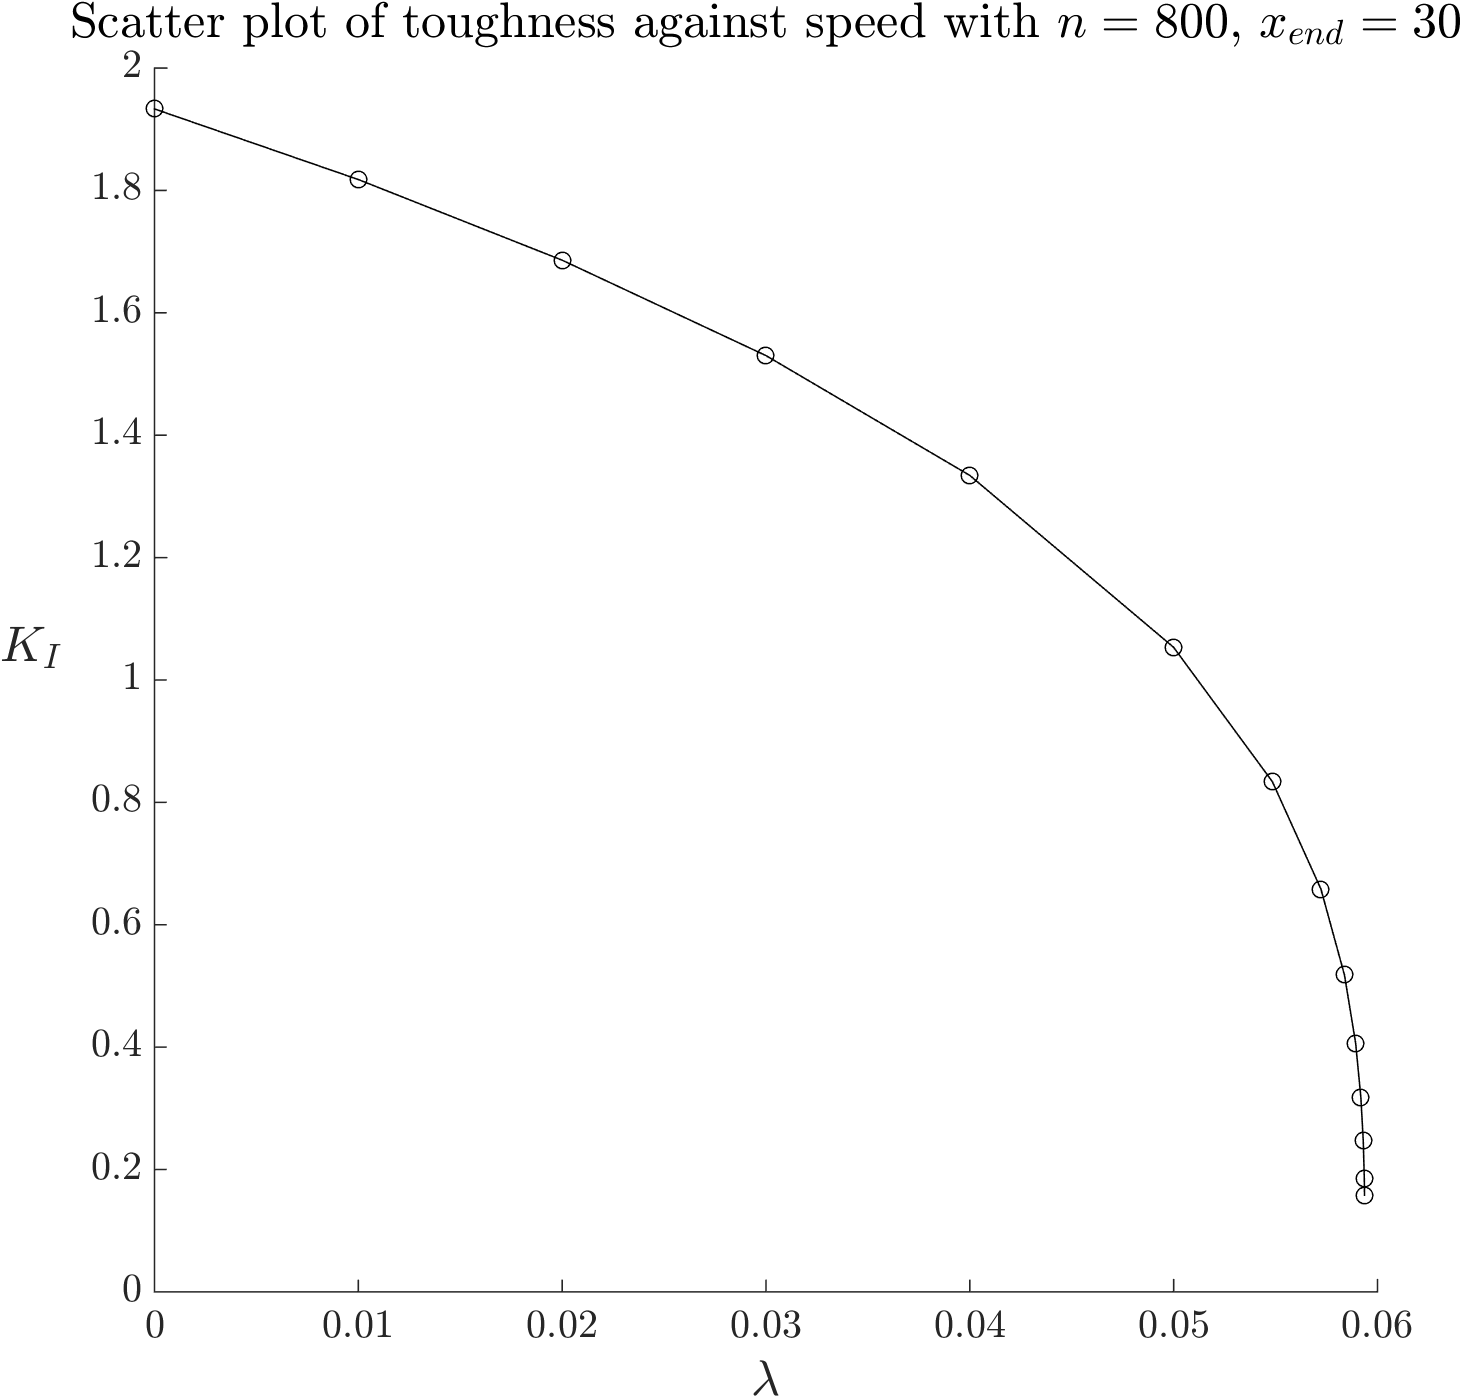
\includegraphics[scale=0.35]{K-lambda.png}
\end{figure}
\begin{figure}[ht]\centering
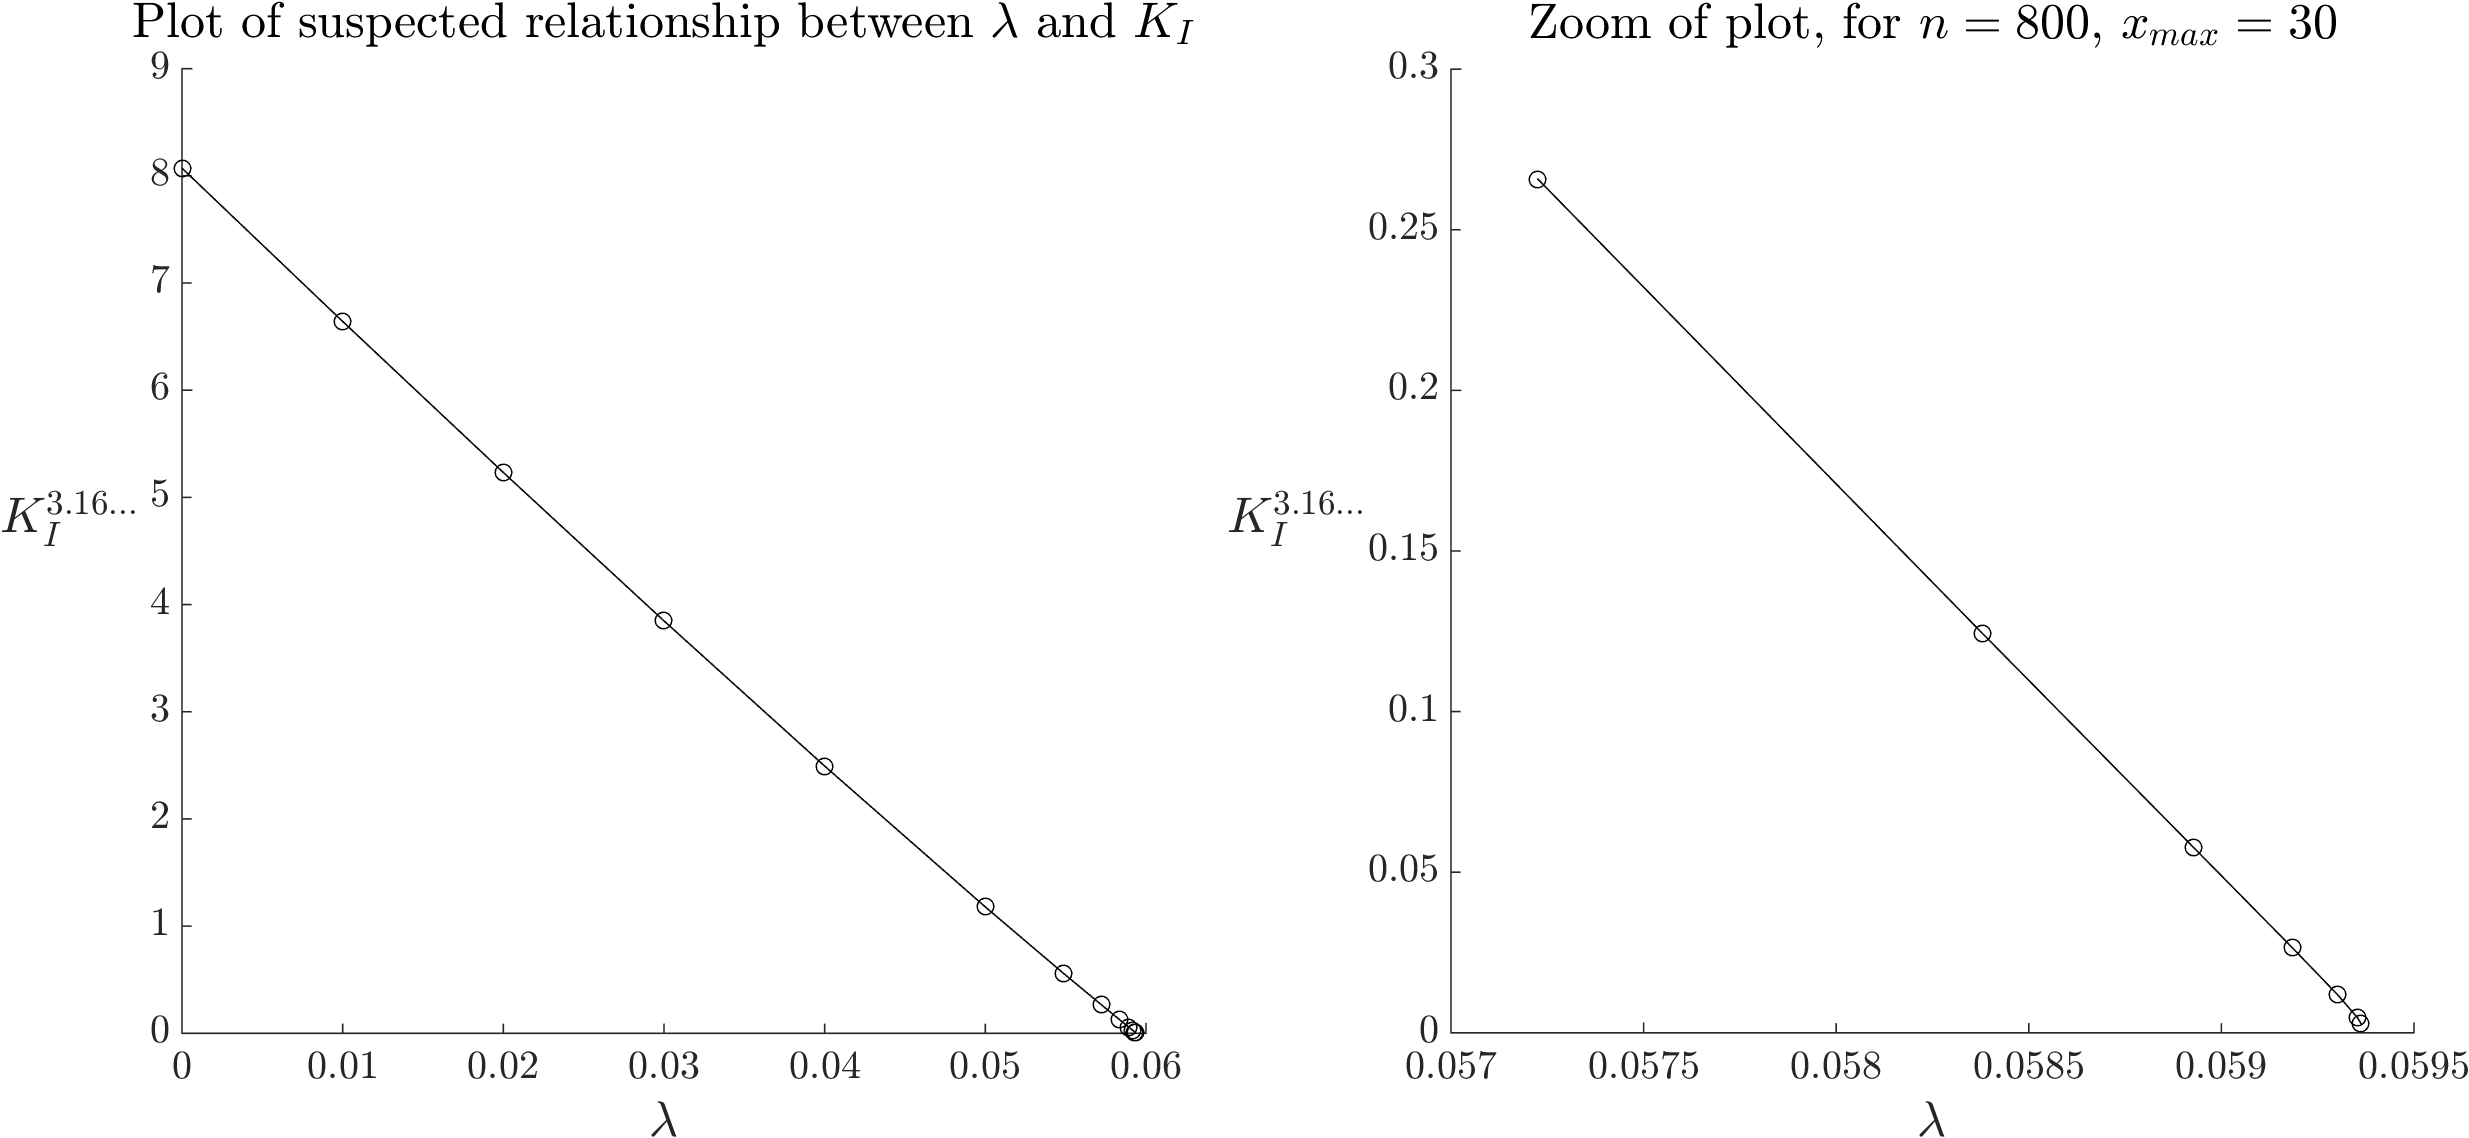
\includegraphics[scale=0.28]{sus-relation.png}
\end{figure}
\clearpage
\begin{figure}[!ht]\centering
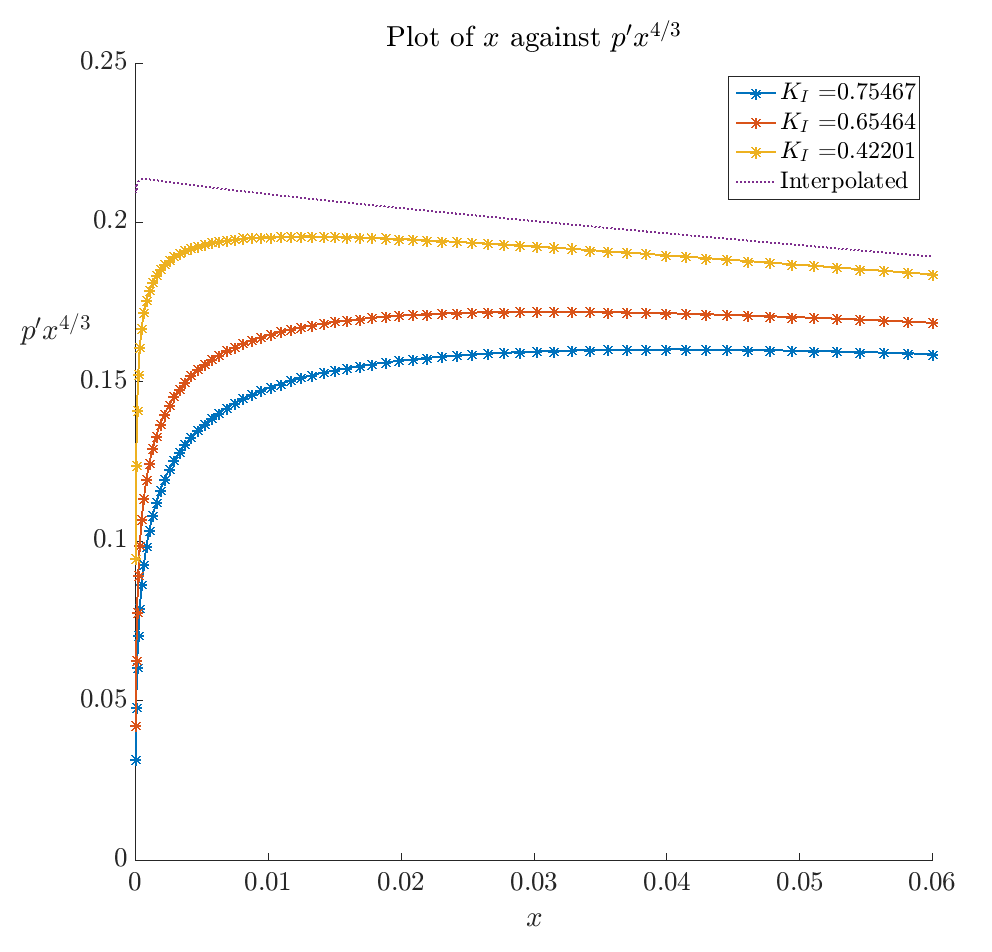
\includegraphics[scale=0.3]{pprime-x.png}
\end{figure}
\begin{figure}[!ht]\centering
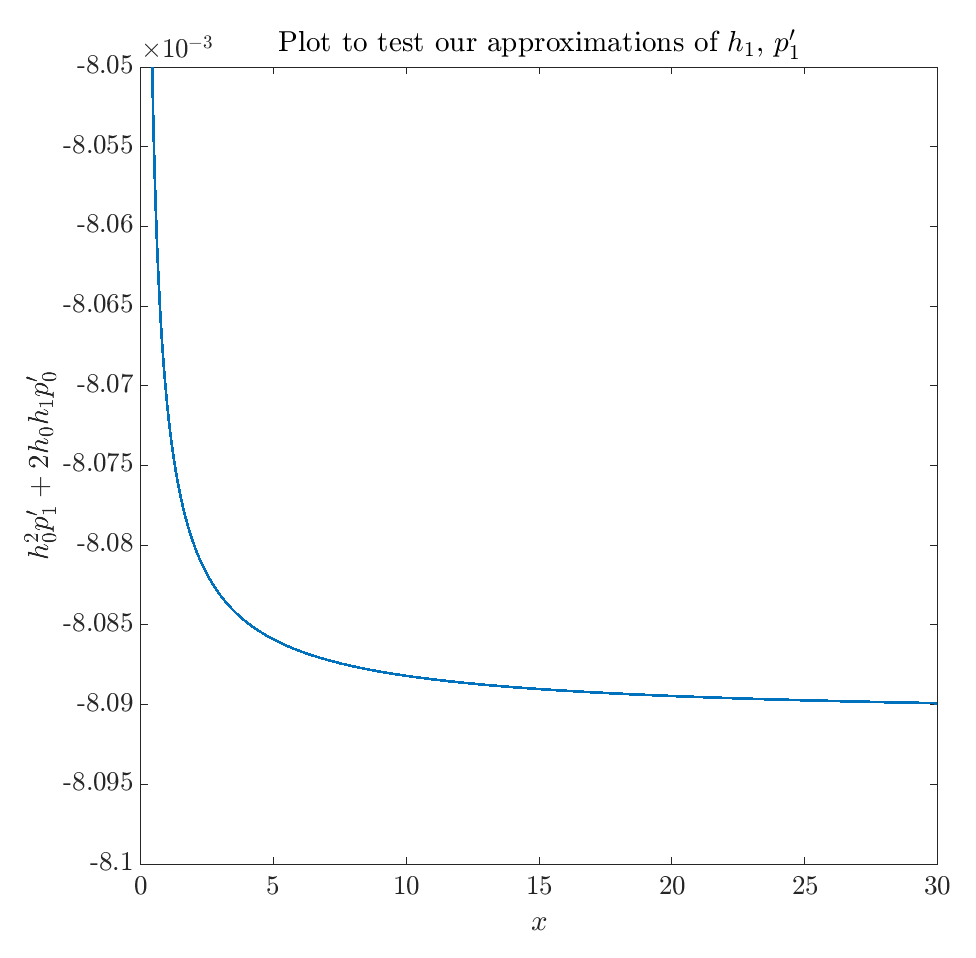
\includegraphics[scale=0.3]{linear-lubrication.png}
\end{figure}
\begin{figure}[!ht]\centering
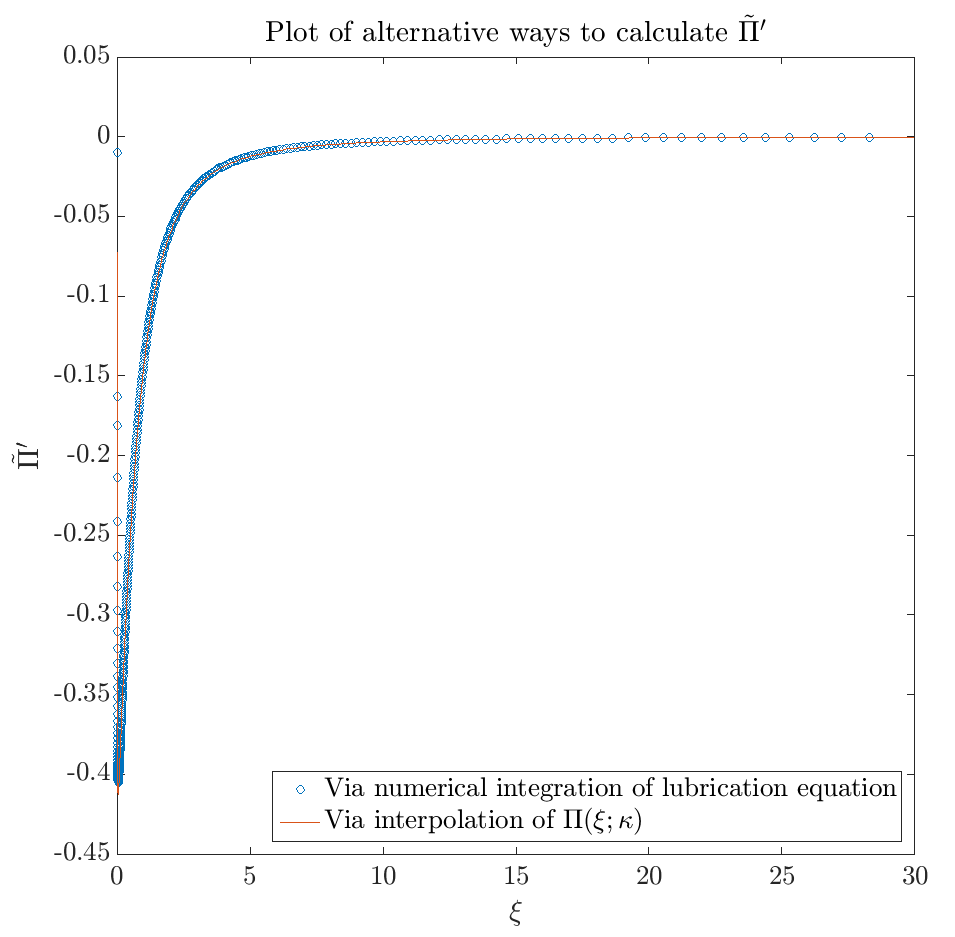
\includegraphics[scale=0.3]{Pi-prime.png}
\end{figure}
\begin{figure}[!ht]\centering
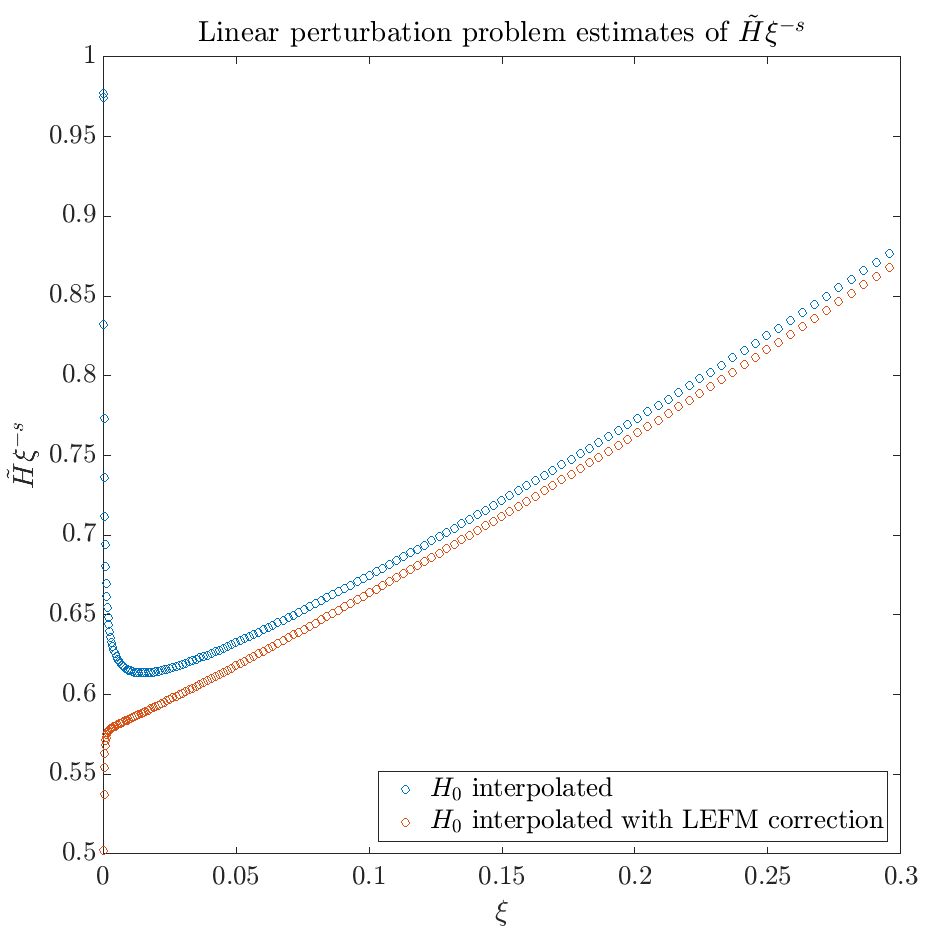
\includegraphics[scale=0.3]{linear-perturb.png}
\end{figure}

\end{document}
